% =====================================================================
% THIS FILE IS THE SOURCE. Edit it, then rebuild the PDF with:
%     bash tools/compile.sh Unit_10_Bayesian_Reasoning_and_Decisions
% (run from the Course_Rewrite folder; it compiles twice and reports
%  page count, overfull boxes, and em dashes)
%
% Do not edit the PDF directly. Figures are the fig_*.pdf files in this
% folder, regenerated by tools/make_module*_slide_figs.py.
%
% Originally converted from the 15-module draft by a one-shot script now
% parked in tools/one_shot_generators/. Re-running those would discard
% anything you change here, so they are kept out of tools/ on purpose.
% =====================================================================
\documentclass[aspectratio=169]{beamer}
\usetheme{default}
\usefonttheme{professionalfonts}
\usepackage{amsmath, amssymb, amsfonts}
\usepackage{graphicx}
\usepackage{booktabs}
\usepackage{bm}
\usepackage{hyperref}

\mode<presentation> {
    \usetheme{Frankfurt}
    \usecolortheme{default}
}

\newcommand{\xbar}{\bar{x}}
\newcommand{\yhat}{\hat{y}}
\newcommand{\PR}[1]{P(#1)}

\newenvironment{principle}[1]{\begin{block}{\textbf{Principle:} #1}}{\end{block}}
\newenvironment{trap}[1]{\begin{alertblock}{\textbf{Trap:} #1}}{\end{alertblock}}
\newenvironment{practice}[1]{\begin{exampleblock}{\textbf{In practice:} #1}}{\end{exampleblock}}
\newenvironment{interview}[1]{\begin{exampleblock}{\textbf{You may be asked:} #1}}{\end{exampleblock}}
\newenvironment{yourturn}[1]{%
  \setbeamercolor{block title}{fg=white,bg=orange!80!black}%
  \setbeamercolor{block body}{bg=orange!12}%
  \begin{block}{\textbf{Your turn:} #1}}{\end{block}}
\newenvironment{livedemo}[1]{%
  \setbeamercolor{block title}{fg=white,bg=teal!80!black}%
  \setbeamercolor{block body}{bg=teal!12}%
  \begin{block}{\textbf{Live demo:} #1}}{\end{block}}
\newenvironment{llmcheck}[1]{%
  \setbeamercolor{block title}{fg=white,bg=violet!75!black}%
  \setbeamercolor{block body}{bg=violet!10}%
  \begin{block}{\textbf{LLM check:} #1}}{\end{block}}

\title{Bayesian Reasoning and Decisions}
\subtitle{Unit 10: Updating Beliefs, and Acting on Them}
\author{Stat 220 \textbar{} Statistics for Data Science}
\date{}

\begin{document}

\begin{frame}
  \titlepage
\end{frame}

% ======================================================================
\section{Why}
% ======================================================================
\begin{frame}{Where this fits}
\begin{itemize}
  \item Everything so far asked: if the null were true, how surprising is this data?
  \item The question people actually ask is the reverse: given this data, what should I now
        believe, and what should I do?
  \item That reversal is Bayes' rule, which you already used for medical tests. Here we apply it to
        the unknown quantity itself: a conversion rate, an effect size, a risk.
\end{itemize}
\begin{principle}{the question you were always trying to answer}
A $p$-value is $\PR{\text{data} \mid \text{hypothesis}}$. A posterior is
$\PR{\text{hypothesis} \mid \text{data}}$. People misread the first as the second constantly,
because the second is what they wanted.
\end{principle}
\end{frame}

\begin{frame}{Live experiment: the two-bag game}
\begin{livedemo}{stand on the probability line}
I have two bags. \textbf{Bag A} is 70\% red chips. \textbf{Bag B} is 30\% red. I have secretly
chosen one, and I will draw chips one at a time, with replacement.
\begin{itemize}
  \item The front wall is a probability line: left end 0\%, right end 100\%.
  \item \textbf{Stand where you think the chance is that I am holding Bag A.} Everyone starts in
        the middle.
  \item After each draw, move. Out loud, one volunteer explains why they moved that far.
\end{itemize}
\end{livedemo}
\vspace{0.2em}
{\tiny\textit{Materials: two opaque bags, about 30 red and 30 white chips, a marked wall or floor line. Time: 12 minutes.}}
\centering\small Five draws. Then we compare where the room stood to where Bayes says it should.
\end{frame}

\begin{frame}{Stay here while they move: the arithmetic}
Starting at 50/50, each red chip multiplies the odds for Bag A by $0.7/0.3 = 2.33$. Each white
chip divides by the same.
\begin{itemize}
  \item After 1 red: \textbf{70\%}. After 2 reds: \textbf{84.5\%}.
  \item A white chip then knocks it back to \textbf{70\%}: exactly one red's worth of evidence,
        undone.
\end{itemize}
\onslide<2->{
Two things the room almost always gets wrong:
\begin{itemize}
  \item People move \textbf{too little} on the first few draws and \textbf{too much} after a long
        streak.
  \item People forget that contradicting evidence subtracts exactly as much as confirming evidence
        adds.
\end{itemize}}
\end{frame}

\begin{frame}{What the game teaches}
\begin{itemize}
  \item Belief is a number that moves, not a verdict you reach.
  \item How far it moves depends on two things only: where you started, and how much more likely
        the data is under one hypothesis than the other.
  \item That ratio, $0.7/0.3$ here, is the \textbf{evidence}. Everything else is bookkeeping.
\end{itemize}
\begin{practice}{the shape of this module}
``How confident are you that the new model is better?'' A Bayesian answer gives a number, and can
say what it would take to change it.
\end{practice}
\end{frame}

\begin{frame}{What this unit gives you}
\begin{columns}[T]
\begin{column}{0.5\textwidth}
\textbf{Things to know}
\begin{itemize}\small
  \item probability as a degree of belief, and when that reading is the useful one
  \item prior, likelihood, and posterior, and how they combine
  \item why the prior matters with little data and washes out with plenty
  \item what a credible interval says, and how it differs from a confidence interval
  \item why Bayesian estimates shrink small groups automatically
  \item how to turn a posterior into a decision using costs
\end{itemize}
\end{column}
\begin{column}{0.5\textwidth}
\textbf{Mistakes to stop making}
\begin{itemize}\small
  \item pretending you have no prior when you obviously do
  \item letting a strong prior drive a conclusion the data cannot support
  \item reading a 95\% confidence interval as a 95\% probability statement
  \item treating a high posterior probability as proof rather than as a bet
  \item forgetting that Bayes assumes your \emph{model} is right
  \item reporting a posterior without saying which prior produced it
\end{itemize}
\end{column}
\end{columns}
\end{frame}

% ======================================================================
\section{Updating}
% ======================================================================
\begin{frame}{Prior, likelihood, posterior}
\[
\underbrace{\PR{\theta \mid \text{data}}}_{\text{posterior}} \;\propto\;
\underbrace{\PR{\text{data} \mid \theta}}_{\text{likelihood}} \times
\underbrace{\PR{\theta}}_{\text{prior}}
\]
\begin{itemize}
  \item The \textbf{prior} is what you believed before: past experiments, industry benchmarks,
        physical limits.
  \item The \textbf{likelihood} is the same object from the estimation module: how well each
        parameter value explains the data.
  \item The \textbf{posterior} is a full distribution over the unknown, not a point. Every question
        you have is answered by an area under it.
\end{itemize}
\end{frame}

\begin{frame}{Updating a rate, with the actual numbers}
Conjugate shortcut: with a Beta$(a, b)$ prior, $s$ successes and $f$ failures give a
Beta$(a+s,\; b+f)$ posterior. The prior acts like $a$ imaginary successes and $b$ imaginary
failures you saw before the study.
\begin{center}\small
\begin{tabular}{lcccc}
\toprule
\textbf{after} & \textbf{data so far} & \textbf{posterior} & \textbf{mean} & \textbf{95\% interval} \\
\midrule
nothing        & none           & Beta(2, 8)     & 0.200 & 0.03 to 0.48 \\
10 visitors    & 2 of 10        & Beta(4, 16)    & 0.200 & 0.07 to 0.40 \\
50 visitors    & 12 of 50       & Beta(14, 46)   & 0.233 & 0.14 to 0.35 \\
200 visitors   & 48 of 200      & Beta(50, 160)  & 0.238 & 0.18 to 0.30 \\
\bottomrule
\end{tabular}
\end{center}
\vspace{0.3em}
\begin{itemize}
  \item The prior contributes 10 imaginary observations. After 200 real ones it is outvoted 20 to
        1, and the interval has shrunk by two thirds.
\end{itemize}
\end{frame}

\begin{frame}{Belief sharpening, batch by batch}
\begin{columns}[c]
\begin{column}{0.58\textwidth}
\centering
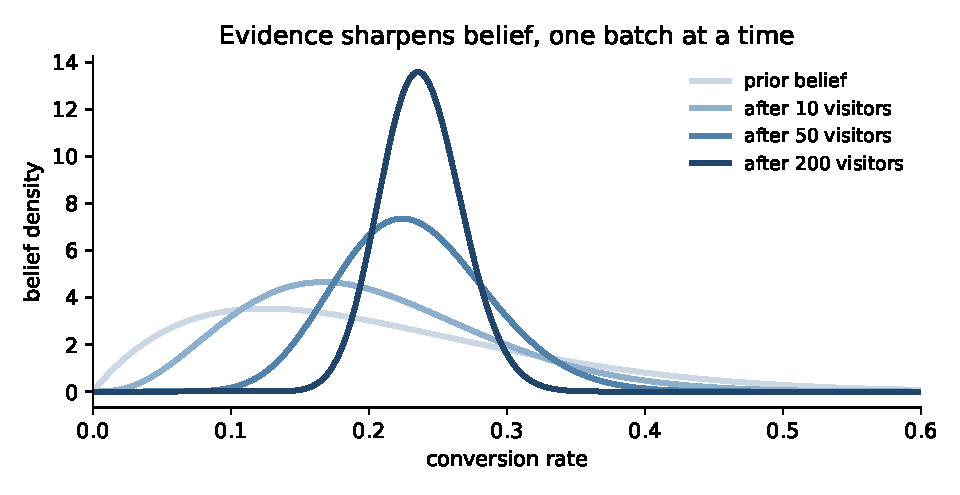
\includegraphics[width=\textwidth]{fig_m13_update.pdf}
\end{column}
\begin{column}{0.42\textwidth}
\small
Estimating a conversion rate, starting from a prior centered near 20\%.
\begin{itemize}
  \item Each batch of visitors narrows the distribution.
  \item Nothing special happens at any threshold. There is no moment of ``significance,'' just
        steadily less uncertainty.
\end{itemize}
\end{column}
\end{columns}
\end{frame}

\begin{frame}{Does the prior take over the answer?}
\begin{center}
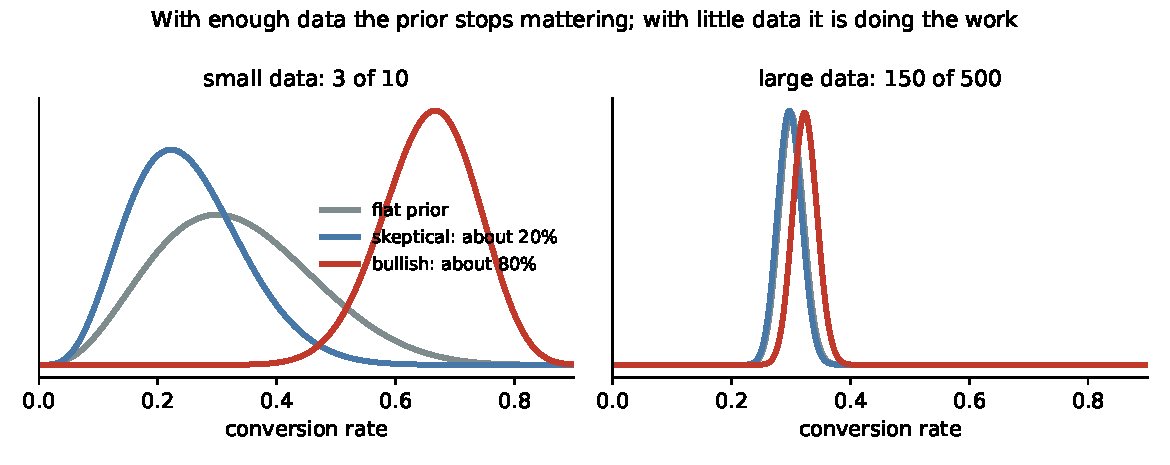
\includegraphics[width=0.92\textwidth]{fig_m13_priors.pdf}
\end{center}
\vspace{-0.4em}
\small
Left: with 10 observations, three reasonable priors give three different answers. Right: with 500,
they are indistinguishable. The prior is a real assumption exactly when the data is thin, which is
exactly when you needed one.
\end{frame}

\begin{frame}{``Isn't the prior just making things up?''}
\begin{itemize}
  \item You already have a prior. When a colleague reports a 400\% conversion lift, you do not
        believe it, and that disbelief is a prior doing its job.
  \item The Bayesian move is to write it down where others can argue with it, instead of applying
        it silently after seeing the result.
  \item The professional practice: use a weak prior, then run a \textbf{sensitivity analysis},
        reporting how the conclusion changes under a skeptical and an optimistic prior.
\end{itemize}
\begin{interview}{how to answer the subjectivity objection}
``Priors are assumptions, and so are the model, the independence, and the choice of test. I would
rather state mine explicitly and show the answer under several of them.''
\end{interview}
\end{frame}

\begin{frame}{Credible intervals versus confidence intervals}
\begin{itemize}
  \item \textbf{Credible interval:} given this data, prior, and model, there is a 95\% probability
        the parameter is in here. That is the sentence everyone wants.
  \item \textbf{Confidence interval:} the procedure that produced this interval captures the truth
        95\% of the time in repeated sampling. The probability is a property of the method.
  \item In practice with plenty of data and a weak prior, the two are usually very close. The
        difference matters most when data is scarce or prior knowledge is strong.
\end{itemize}
\begin{trap}{the universal misreading}
Nearly everyone reads a confidence interval as a credible interval. If that is the statement you
want, say so, use a prior, and earn it.
\end{trap}
\end{frame}

% ======================================================================
\section{Decisions}
% ======================================================================
\begin{frame}{A Bayesian A/B test}
\begin{columns}[c]
\begin{column}{0.6\textwidth}
\centering
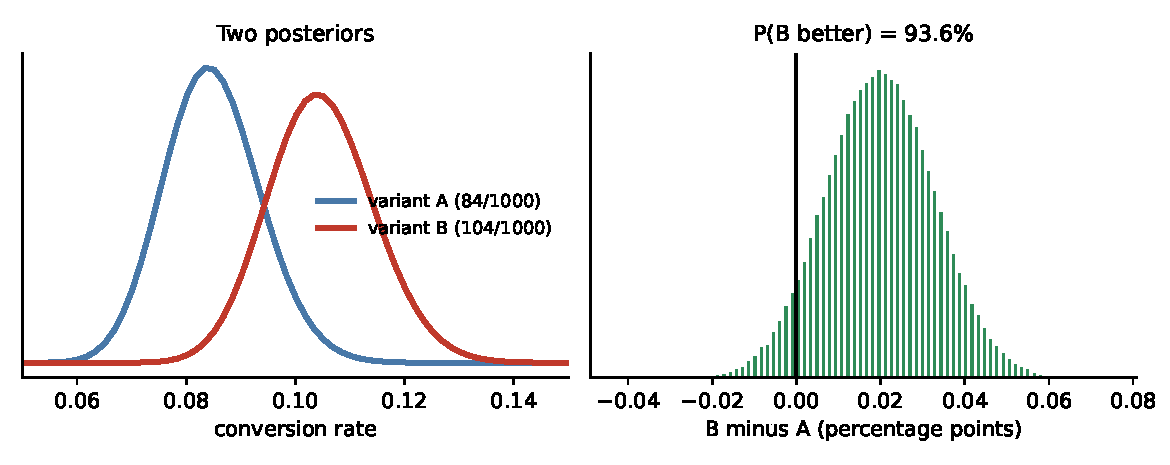
\includegraphics[width=\textwidth]{fig_m13_ab.pdf}
\end{column}
\begin{column}{0.4\textwidth}
\small
1{,}000 visitors each: A converts 84, B converts 104.
\begin{itemize}
  \item $\PR{\text{B better than A}} = \textbf{93.6\%}$.
  \item The same data gives a frequentist $p = 0.125$, which most people read as ``not significant.''
\end{itemize}
\end{column}
\end{columns}
\onslide<2->{\centering\small
Both are correct. They answer different questions, and only one of them is the question the product
manager asked.}
\end{frame}

\begin{frame}{From posterior to decision: expected loss}
\begin{itemize}
  \item Do not stop at ``93.6\% likely better.'' Ask what it costs to be wrong.
  \item \textbf{Expected loss} of shipping B: average, over the posterior, of how much worse B is
        whenever it is worse. Here that is about \textbf{0.04 percentage points} of conversion.
  \item If 0.04 points is negligible relative to the upside, ship. The decision rule is a cost
        comparison, not a threshold on probability.
\end{itemize}
\begin{principle}{the deliverable is an action with its expected cost}
``Ship B. The chance we are wrong is 6\%, and the expected cost if we are is tiny compared with the
expected gain'' is a complete answer.
\end{principle}
\end{frame}

\begin{frame}{Shrinkage, for free}
\begin{columns}[c]
\begin{column}{0.6\textwidth}
\centering
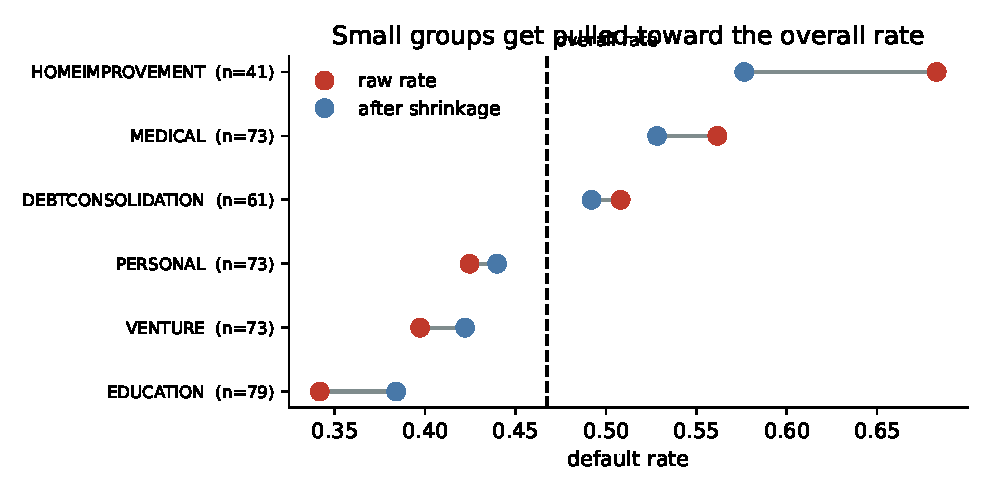
\includegraphics[width=\textwidth]{fig_m13_shrinkage.pdf}
\end{column}
\begin{column}{0.4\textwidth}
\small
Default rates by loan purpose in a 400-loan sample.
\begin{itemize}
  \item Small categories have wild raw rates.
  \item A prior centered on the overall rate pulls them in, by an amount that depends on their
        sample size.
\end{itemize}
This is the leaderboard fix from the estimation module, arising automatically.
\end{column}
\end{columns}
\end{frame}

\begin{frame}{Your turn \#1}
\begin{yourturn}{how much do you believe it?}
A colleague reports an A/B test on a checkout button: \textbf{240\% lift} in conversion, $p = 0.03$,
based on 60 visitors per arm.
\vspace{0.3em}

With a neighbor: what is your posterior belief that the true lift exceeds 100\%? What prior are you
using, and what would change your mind?
\end{yourturn}
\end{frame}

\begin{frame}{Your turn \#1: answer}
\begin{itemize}
  \item Your prior, built from every A/B test ever run, says real button changes move conversion by
        a few percent, not by 240\%.
  \item With 60 visitors per arm the likelihood is very flat, so it barely moves that prior. The
        posterior stays near ``a small effect, if any.''
  \item This is the winner's curse in Bayesian language: extreme estimates from tiny samples are
        mostly noise, and a sensible prior discounts them automatically.
  \item What would change your mind: a preregistered replication at ten times the sample size.
\end{itemize}
\begin{principle}{extraordinary claims need extraordinary likelihood ratios}
The more surprising the claim, the more evidence it takes to move you. That is arithmetic, not stubbornness.
\end{principle}
\end{frame}

\begin{frame}{Your turn \#3}
\begin{yourturn}{how much would this move you?}
Your company's landing pages historically convert between 6\% and 14\%. A new page is tested and
converts \textbf{4 of 10} visitors, which is 40\%.
\vspace{0.3em}

With a neighbor: pick a prior that encodes the company history, work out roughly where the
posterior lands, and decide what you would tell the person who wants to ship it today.
\end{yourturn}
\end{frame}

\begin{frame}{Your turn \#3: answer}
\begin{itemize}
  \item A prior centered near 10\% with real weight, say Beta(10, 90), encodes ``about 10\%, worth
        roughly 100 past observations.''
  \item Posterior: Beta$(10+4,\; 90+6) =$ Beta(14, 96), a mean near \textbf{12.7\%}. The
        spectacular 40\% barely moves the needle, because 10 visitors is almost no evidence.
  \item What to say: ``This is encouraging but it is 10 people. Our best estimate is still about
        13\%. Run it to a few thousand visitors before we decide.''
\end{itemize}
\begin{principle}{the winner's curse, in Bayesian clothing}
A sensible prior automatically discounts extreme results from tiny samples. That is not conservatism. It is what the
arithmetic says once you admit you knew something beforehand.
\end{principle}
\end{frame}

\begin{frame}{When to stop a test}
\begin{itemize}
  \item In the frequentist frame, peeking at a $p$-value and stopping when it dips below 0.05
        inflates the false-positive rate badly. You saw this in Part 1.
  \item A posterior can be looked at any time without that particular problem, because it is a
        statement about current belief rather than a long-run error rate.
  \item But it is not a free lunch: if you stop the moment the posterior crosses a threshold, you
        still systematically overstate the effect. Use a decision rule based on \textbf{expected
        loss} and a planned horizon.
\end{itemize}
\begin{trap}{``Bayesian methods let you peek''}
They let you look. They do not protect you from stopping early on a lucky run and shipping an
inflated estimate.
\end{trap}
\end{frame}

\begin{frame}{Your turn \#2}
\begin{yourturn}{price the information}
You are deciding whether to launch in a new city. Launching costs \$400k. Your posterior says a
60\% chance of a \$1M return and a 40\% chance of \$0.
\vspace{0.3em}

With a neighbor: (i) should you launch? (ii) A market study costing \$50k would tell you which case
you are in with high accuracy. Is it worth buying?
\end{yourturn}
\end{frame}

\begin{frame}{Your turn \#2: answer}
\begin{itemize}
  \item (i) Expected return is $0.6(1{,}000) + 0.4(0) = \$600$k against a \$400k cost, so the
        expected profit is \textbf{+\$200k}. Launch, if you can absorb the 40\% chance of losing
        \$400k.
  \item (ii) With a perfect study you launch only in the good case: expected profit
        $0.6 \times \$600\text{k} = \$360$k. The study is worth up to
        $\$360 - \$200 = \textbf{\$160k}$, so \$50k is a good buy.
\end{itemize}
\begin{principle}{information has a computable price}
The value of a study is the improvement in your expected outcome from being able to act on what it
tells you. If a study cannot change your decision, its value is zero, no matter how interesting it
is.
\end{principle}
\end{frame}

% ======================================================================
\section{LLM check}
% ======================================================================
\begin{frame}{LLM check: mistake or not? (1 of 2)}
\begin{llmcheck}{we asked an LLM to interpret an interval}
\textbf{We told it:} ``Our 95\% confidence interval for the treatment effect is 2 to 8. What does
that mean?''\\[4pt]
\textbf{It answered:} ``There is a 95\% probability that the true treatment effect is between 2 and
8.''
\end{llmcheck}
\vspace{0.2em}
\centering\small Mistake, or no mistake?
\onslide<2->{%
\begin{trap}{verdict: mistake}
That is the definition of a \emph{credible} interval. A confidence interval says the procedure
captures the truth 95\% of the time across repeated samples. The parameter is not treated as
random. The two often nearly coincide, but the sentence as written is the classic misreading.
\end{trap}}
\end{frame}

\begin{frame}{LLM check: mistake or not? (2 of 2)}
\begin{llmcheck}{same territory, a different answer}
\textbf{We told it:} ``We have 12 sales from a brand-new region. The conversion rate looks like
40\%, way above our 9\% average. Should we expand there?''\\[4pt]
\textbf{It answered:} ``With 12 observations that 40\% carries enormous uncertainty. I would shrink
it toward the 9\% company average using a prior built from your other regions, which will land the
estimate closer to 12--15\%, and I would treat expansion as a decision under uncertainty: what does
it cost if the true rate is 9\%?''
\end{llmcheck}
\vspace{0.2em}
\centering\small Mistake, or no mistake?
\onslide<2->{%
\begin{principle}{verdict: no mistake}
Prior from related data, shrinkage proportional to sample size, and a decision framed by costs.
That is this unit in three sentences.
\end{principle}}
\end{frame}

% ======================================================================
\section{Workflow}
% ======================================================================
\begin{frame}{The arc of a Bayesian analysis}
\begin{enumerate}
  \item \textbf{Write the unknown in words} and what decision depends on it.
  \item \textbf{State a prior} from past data or domain knowledge, and say where it came from.
  \item \textbf{Write the likelihood}, which is just your model of how the data arises.
  \item \textbf{Compute the posterior}, by formula in simple cases and by simulation otherwise.
  \item \textbf{Summarize what matters}: the credible interval, and the probability of the
        statements someone actually cares about.
  \item \textbf{Attach costs and choose an action}, reporting the expected loss.
  \item \textbf{Run a sensitivity check} under a skeptical and an optimistic prior.
\end{enumerate}
\end{frame}

\begin{frame}{Scenario: the executive who wants one number}
\textbf{Setup.} You present a posterior. The VP says: ``Just tell me, does it work or not?''
\begin{itemize}
  \item Give the decision, not the distribution: ``Yes, ship it. There is a 94\% chance it is
        better, and if we are wrong the cost is about \$8k a month, against an expected gain of
        \$140k.''
  \item Then offer the caveat that could change the call: ``This assumes next quarter looks like
        last quarter. If the seasonal mix shifts, I would re-check in six weeks.''
  \item Keep the distribution in the appendix, for the people who will ask.
\end{itemize}
\begin{principle}{translate, do not simplify}
Executives are not asking you to discard uncertainty. They are asking you to convert it into a
recommendation with a stated risk.
\end{principle}
\end{frame}

% ======================================================================
\section{Consolidate}
% ======================================================================
\begin{frame}{From prior to decision}
\small
\begin{enumerate}
  \item \textbf{Write the unknown in words} and say what decision depends on it.
  \item \textbf{State a prior} from past data, and say where it came from.
  \item \textbf{Update.} For a rate, a Beta$(a,b)$ prior with $s$ successes and $f$ failures becomes Beta$(a+s,\,b+f)$.
  \item \textbf{Summarize the posterior}: the mean, and a credible interval from the 2.5 and 97.5 percentiles.
  \item \textbf{Answer the question actually asked}, such as $\PR{\text{B beats A}}$, by drawing from both posteriors and comparing.
  \item \textbf{Attach costs} and compute the expected loss of each action.
  \item \textbf{Re-run under a skeptical and an optimistic prior} and report whether the decision changes.
\end{enumerate}
\end{frame}

\begin{frame}{The traps, all in one place}
\begin{trap}{the ones that bite most often}
\begin{itemize}
  \item Claiming you have no prior.
  \item Letting a confident prior overwhelm data it should have updated on.
  \item Reading a confidence interval as a probability about the parameter.
  \item Treating a 95\% posterior as certainty rather than a one-in-twenty bet.
  \item Forgetting that Bayes assumes the model, not just the prior.
  \item Stopping a test the moment the posterior crosses a line.
  \item Reporting a posterior without naming the prior behind it.
\end{itemize}
\end{trap}
\end{frame}

\begin{frame}{Ten questions to be able to answer}
\begin{enumerate}\small
  \item Explain prior, likelihood, and posterior with an example from your own work.
  \item What is the probability variant B is better, and how is that different from a $p$-value?
  \item Is choosing a prior unscientific? Defend your practice.
  \item Credible interval versus confidence interval: state both precisely.
  \item We have 12 observations from a new market. How do you estimate the rate?
  \item How do you turn a posterior into a ship-or-not decision?
  \item What is expected loss, and why report it alongside a probability?
  \item Can you peek at a Bayesian test whenever you like? Explain carefully.
  \item How much is a market study worth, and when is it worth nothing?
  \item A colleague reports a 240\% lift from 60 users. What is your posterior?
\end{enumerate}
\end{frame}

\begin{frame}{Mastery checklist}
You have this unit when you can, from memory:
\begin{itemize}
  \item state Bayes' rule for a parameter and name each piece
  \item explain when the prior matters and when it washes out
  \item interpret a credible interval correctly and contrast it with a confidence interval
  \item explain why Bayesian estimates shrink small groups
  \item compute the probability of a business-relevant statement from a posterior
  \item convert a posterior into a decision with an expected loss
  \item run and report a sensitivity analysis over priors
\end{itemize}
\end{frame}

\begin{frame}{What you should be able to do with software}
\small
Nobody is asking you to memorize syntax. You are expected to know \emph{which} procedure the
question calls for, what to hand it, and what the output means. With an AI assistant open, you
should be able to produce any of these and defend the result.
\begin{center}\footnotesize
\begin{tabular}{p{0.44\textwidth} p{0.46\textwidth}}
\toprule
\textbf{You should be able to} & \textbf{What you would reach for} \\
\midrule
Posterior for a rate & \texttt{stats.beta(a+s, b+f)} \\
Credible interval & \texttt{posterior.ppf([0.025, 0.975])} \\
Draw from a posterior & \texttt{posterior.rvs(200\_000)} \\
Probability one variant beats another & \texttt{(draws\_b > draws\_a).mean()} \\
Expected loss of a decision & \texttt{np.maximum(a - b, 0).mean()} \\
Shrunken group estimates & \texttt{(successes + k*p\_bar) / (n + k)} \\
Value of a study & simulate deciding with and without it, and difference the profits \\
\bottomrule
\end{tabular}
\end{center}
\vspace{0.2em}
\centering\small
If you cannot say what the output means, the fact that you produced it is worth nothing.
\end{frame}

\begin{frame}{Where we go next}
\begin{itemize}
  \item One thing remains, and it is the one that decides whether any of this matters: where the
        data came from in the first place.
  \item Next part: \textbf{sampling, selection, and missing data}, the failures that no model,
        prior, or test can repair.
\end{itemize}
\begin{principle}{the through-line}
Evidence updates belief. Belief plus costs makes a decision. Being explicit about all three is what
separates an analyst from a calculator.
\end{principle}
\end{frame}

\end{document}
